\section{Visual Quality Guaranteed Sampling Approach}
Due to the hardness of the Problem~\ref{prob:def}, we first introduce a straight-forward solution for it in Section~\ref{sec:random}.
Then, we propose a visual quality guaranteed sampling approach in Section~\ref{sec:greedy}.
Last, we devise several optimizations to improve the efficiency and effectiveness of our proposal in Section~\ref{sec:opt}.


\subsection{Uniform Random Sampling Algorithm}~\label{sec:random}
The straight forward solution for Problem~\ref{prob:def} is uniform random sampling.
As the pseudocode in Algorithm~\ref{alg:rand} shown, it randomly selecting $k$ trajectories from $\D$, then render these selected $k$ trajectories into the canvas.

\begin{algorithm}
    \caption{RandSampling($\D$,k)} \label{alg:rand}
    \begin{algorithmic}[1]
    \State Initialize result set $\oR \leftarrow \emptyset$
    \While{$|\oR| < k$}
        \State $\oR_{tmp} \leftarrow \mathsf{RAND(\D-\oR)}$
        \State $\oR \leftarrow \oR \cup \{ \oR_{tmp} \}$
    \EndWhile
    \State Return $\oR$
    \end{algorithmic}
\end{algorithm}

Obviously, the uniform random sampling algorithm has good performance.
However, it does not provide any guarantee on the visual quality of the visualization result.


%Trajectory data $\D$\cite{xxx} consists of almost 10K trajectories which collected by Didi company.
%The visualization result of the whole dataset $\D$ is illustrated in Figure~\ref{fig:demo}(b).
%Figure~\ref{fig:demo}(b) shows the visualization result of uniform random sampling result of $\D$ with $k=100$.
%The difference between the visualization results in Figures~\ref{fig:demo}(a) and (b) are obvious from user's perspective.

%\begin{figure}
% \centering
% \small
% \begin{tabular}{cc}
%   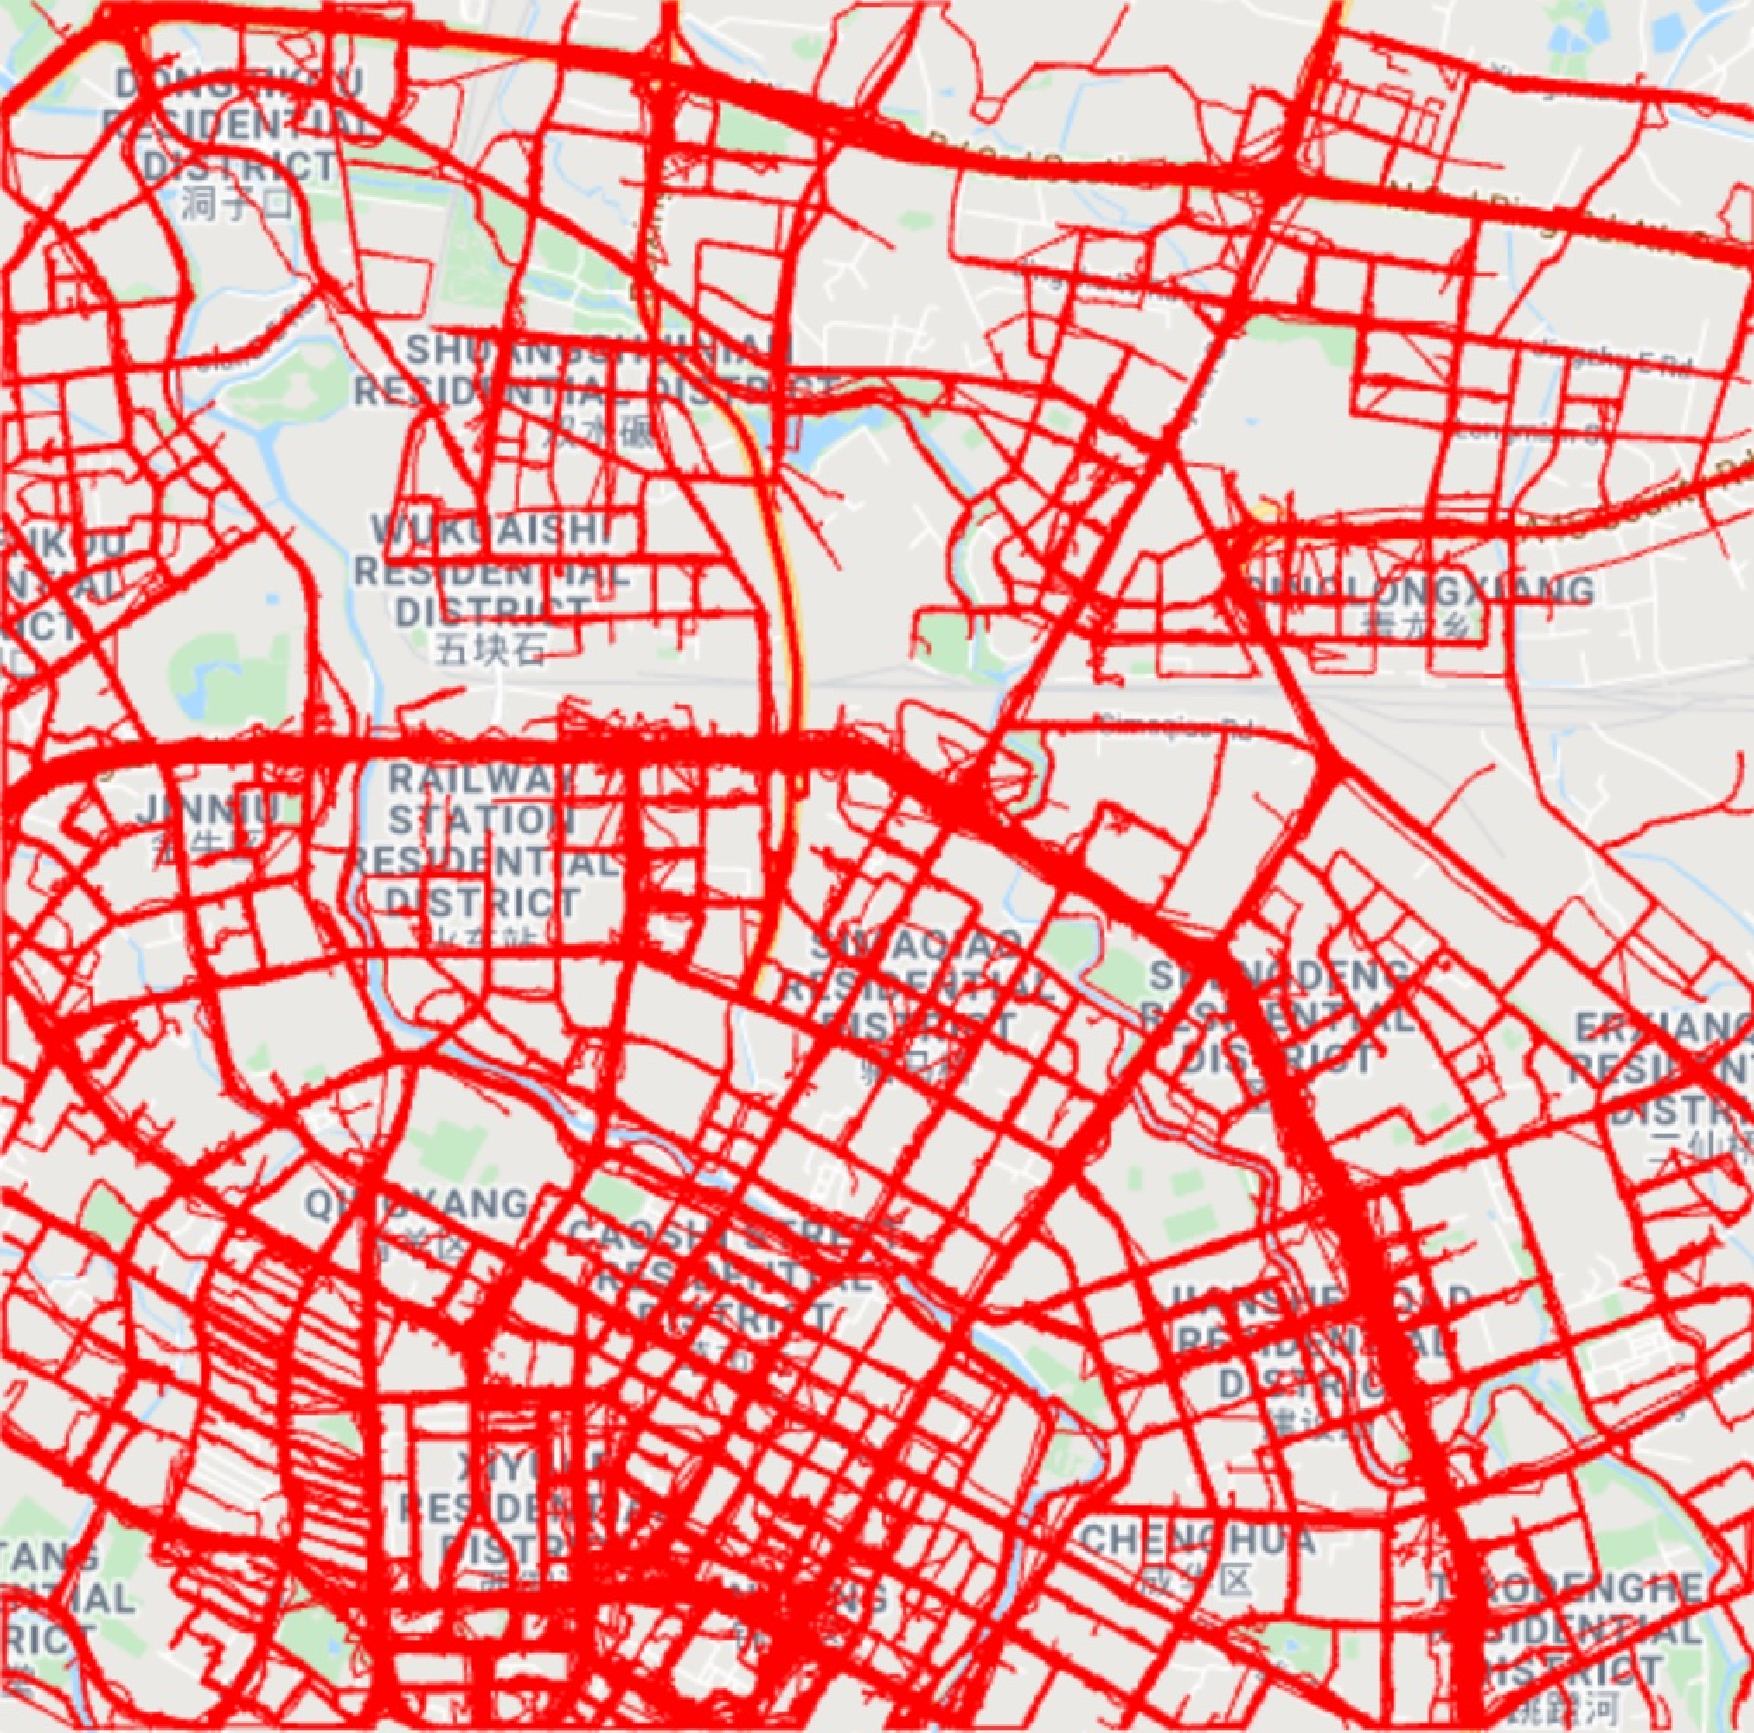
\includegraphics[width=0.45\columnwidth]{chengdu_total}
%   &
%   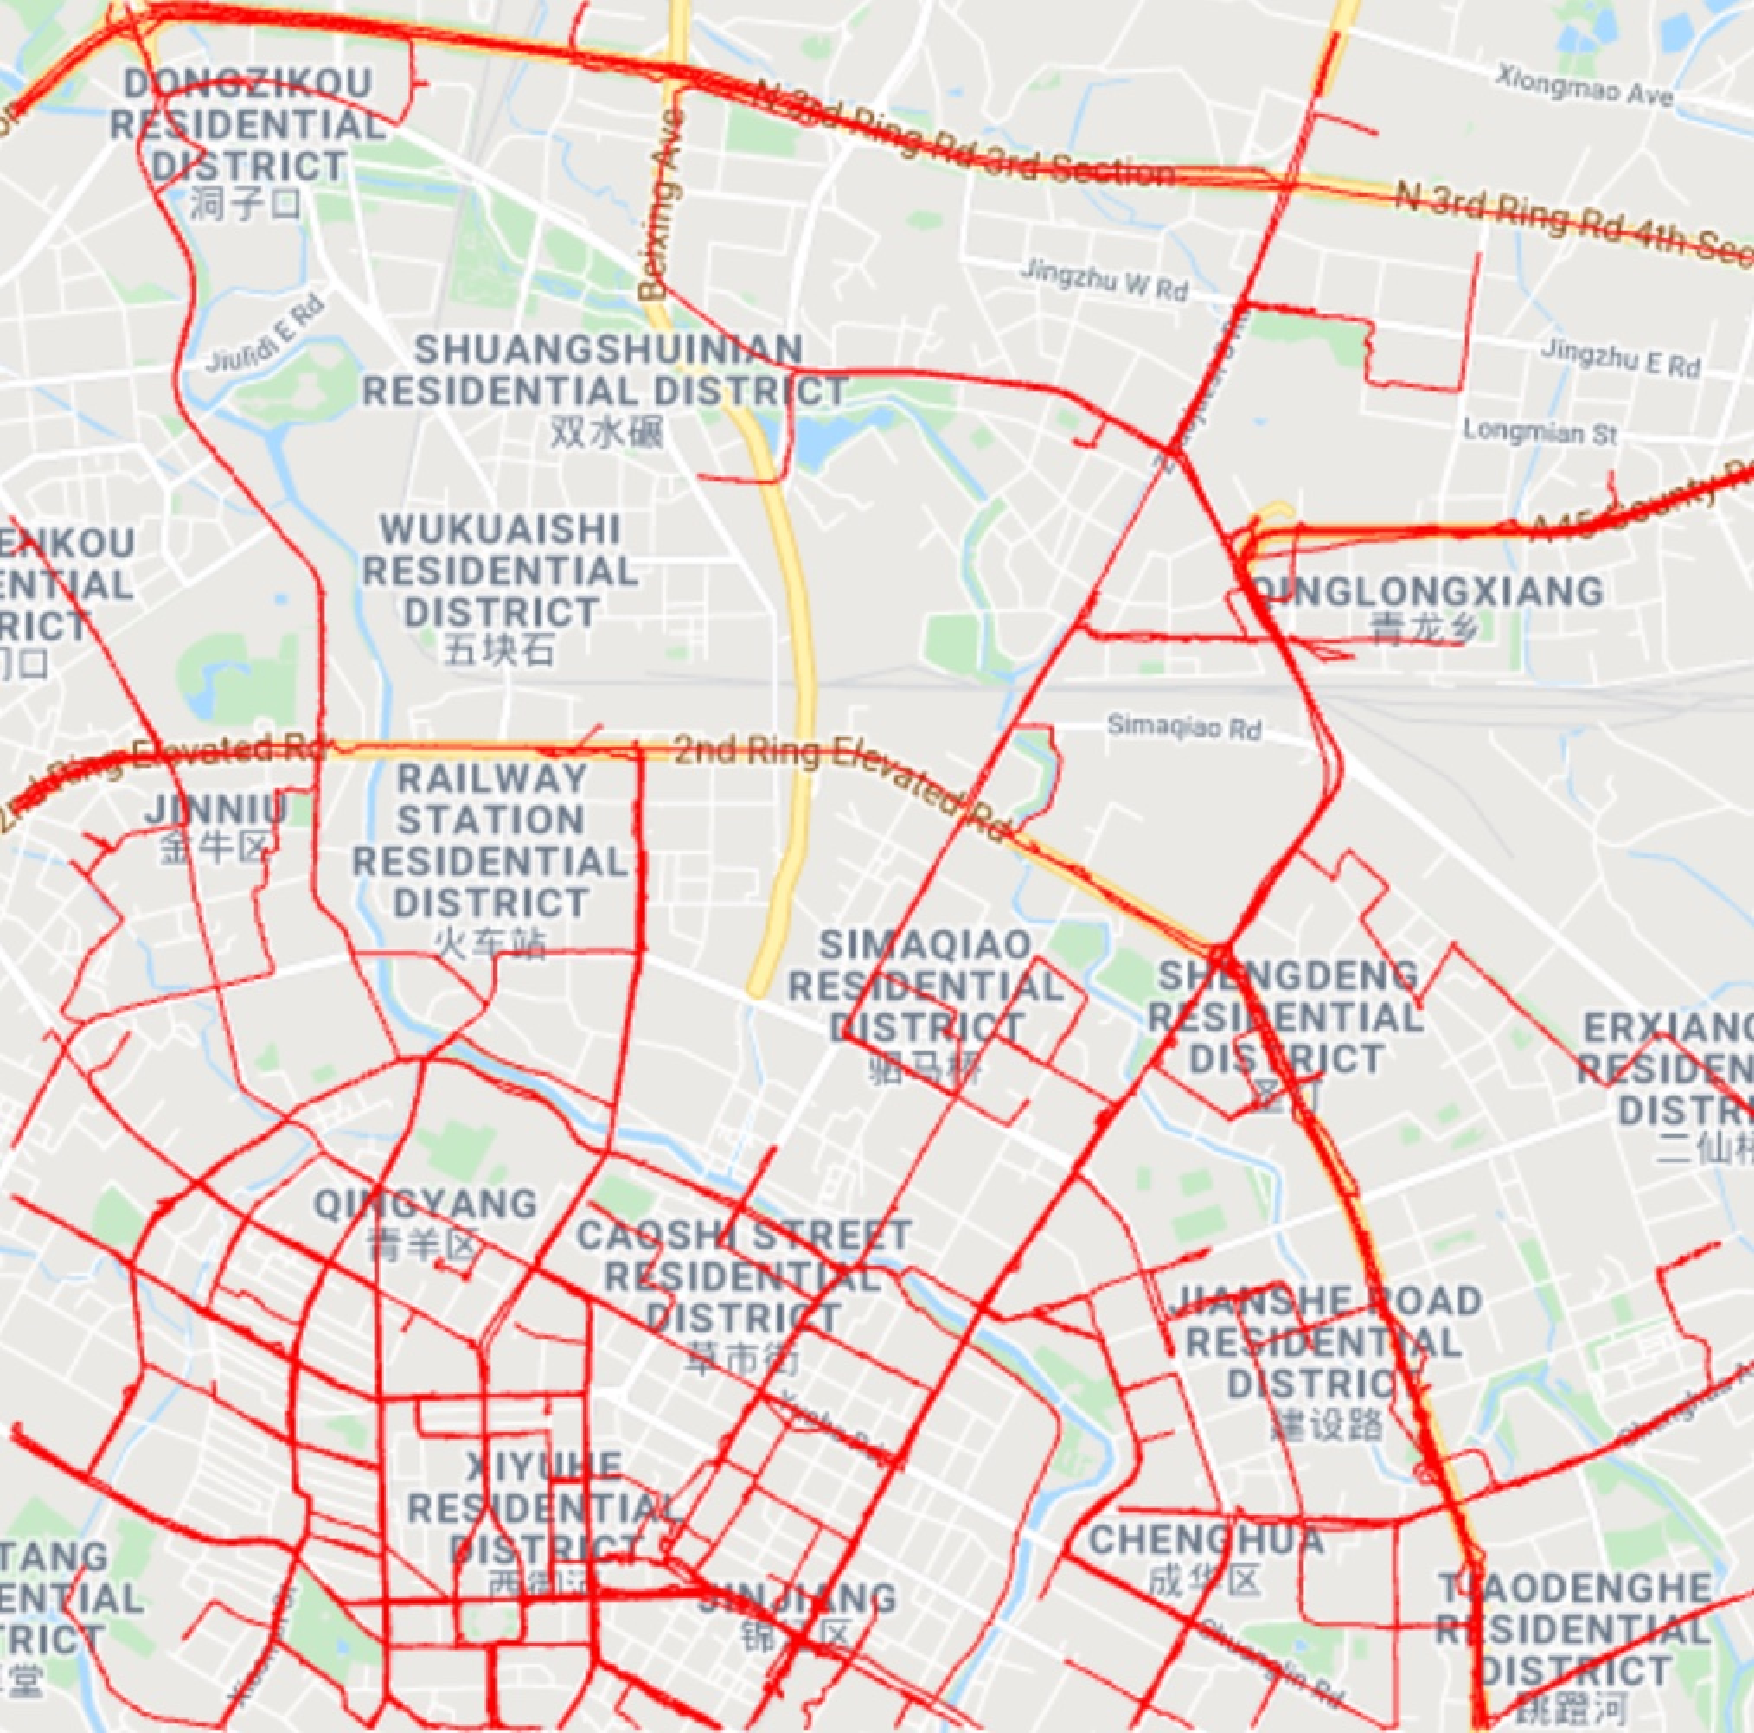
\includegraphics[width=0.45\columnwidth]{chengdu_sampling}
%   \\
%   (a) Dataset $\D$
%   &
%   (b) Uniform sampling $\oR$
% \end{tabular}
% \caption{Visualization results of trajectory set in Chengdu}
% \label{fig:demo}
%\end{figure}

\subsection{Visual Quality Guaranteed Sampling Algorithm}~\label{sec:greedy}
In this section, we present our visual quality guaranteed sampling algorithm for Problem~\ref{prob:def}.
We start our presentation by elaborating the relationship between visual quality of sampled set $\oR$ and user zoom level.
Obviously, for a given sampled set $\oR \subseteq \D$, it has different loss values at different user zoom level.
%The reason is the pixel size will be updated at different zoom level.
\QM{The reason is the map are of the same canvas region will be updated at different zoom level.}
For example, Google map\footnote{\url{https://www.google.com/maps/preview}} provides zoom levels range from 0 to 20,
where level 0 is the lowest level (e.g., the whole world), level 20 is the highest level (e.g., individual building, if available).
In order to devise a zoom level oblivious visualization for sampled dataset $\oR$,
we use the highest zoom level to define the size of each pixel in the canvas in our problem.
For each trajectory $\D_i in \D$ is a set of pixels at highest zoom level in the canvas.

The visual quality guaranteed sampling algorithm employs greedy paradigm.
In particular, it finds the trajectory $\D_i$ in $\D$ which maximize the union set of $\oR \cup \D_i$ at each iteration, as Line~\ref{line:max} shown in Algorithm~\ref{alg:greedy}.
It terminates after $k$ iterations and returns $\oR$ as result set for rendering.

\begin{algorithm}
    \caption{VQGS($\D$,k)} \label{alg:greedy}
    \begin{algorithmic}[1]
    \State Initialize result set $\oR \leftarrow \emptyset$
    \While{$|\oR| < k$}
        \State $\oR_{tmp} \leftarrow argmax_{\D_i \in \D} \oR \cup \D_i$ \label{line:max}
        \State $\oR \leftarrow \oR \cup \{ \oR_{tmp} \}$
    \EndWhile
    \State Return $\oR$
    \end{algorithmic}
\end{algorithm}

Interestingly, Algorithm~\ref{alg:greedy} has a nice theoretical property, i.e., it guarantees the visual quality of the returning set $\oR$, as proved in Theorem~\ref{the:ratio}.

\begin{theorem}~\label{the:ratio}
Algorithm~\ref{alg:greedy} provides $1-(1-1/k)^k \geq (1-1/e) \approx 0.632$ approximation result for large trajectory visualization problem (i.e., Problem~\ref{prob:def}).
\end{theorem}

\begin{proof}
The optimal solution of Problem~\ref{prob:def} covers $OPT$ elements in $k$ iterations.
Let $a_i$ be the number of newly covered elements at the $i$-th iteration, $b_i$ is the total number of covered elements up to the $i$-th iteration (i.e., $b_i = \sum_{j=1}^{i}a_i$),
and $c_i$ be the uncovered elements after $i$-th iteration (i.e., $c_i = OPT-b_i$).
According to greedy paradigm, we can conclude the number of newly covered elements at the $(i+1)$-th iteration is always greater than or equal to $\frac{1}{k}$ of the number of uncovered elements after the $i$-th iteration, i.e., $a_{i+1} \geq \frac{c_i}{k}$.
We prove Theorem~\ref{the:ratio} by proving $c_{i+1} \leq (1-1/k)^{i+1} \cdot OPT$.
It holds $c_1 \leq (1-1/k) \cdot OPT$ as follows.
\begin{align} \nonumber
& a_1 \geq c_0 \cdot 1/k = 1/k \cdot OPT \text{~~~as we concluded~~~} a_{i+1} \geq \frac{c_i}{k}\\ \nonumber
 \Leftrightarrow  & b_1 \geq 1/k \cdot OPT  \Leftrightarrow  -b_1 \leq - 1/k \cdot OPT  \text{~~~as~~~} a_1 = b_1\\ \nonumber
 \Leftrightarrow & OPT - b_ 1 \leq OPT - 1/k \cdot OPT  \Leftrightarrow  c_1 \leq (1-1/k) \cdot OPT
\end{align}
For inductive hypothesis assume $c_{i} \leq (1-1/k)^i \cdot OPT$. Thus,
\begin{align} \nonumber
& c_{i+1} = c_i - a_{i+1} \leq c_i - c_i/k = (1-1/k) \cdot c_i = (1-1/k)^{i+1} \cdot OPT
\end{align}

Hence, it holds $c_k \leq (1-1/k)^{k} \cdot OPT$.
It is equivalent to $b_k \geq (1 - (1-1/k)^{k}) \cdot OPT \geq (1-1/e) \cdot OPT \approx 0.632 \cdot OPT$.
\end{proof}


\subsection{Optimization Techniques}~\label{sec:opt}
With the above analysis, Algorithm~\ref{alg:greedy} provides a visual quality guaranteed sampling algorithm for large trajectory data visualization problem.
However, it is impractical for (very) large trajectory dataset (i.e., billions of trajectories) as the time complexity analyzed in the following Lemma~\ref{lem:cost}.

\begin{lemma}[Time Complexity]~\label{lem:cost}
Given trajectory dataset $\D$ and an integer $k$, the time complexity of Algorithm~\ref{alg:greedy} is $O(k \cdot m \cdot |\D|)$, where $m$ is the maximum length of the trajectory in dataset $\D$.
\end{lemma}

\begin{proof}
The complexity analysis is straight forward as all trajectories (i.e., $|\D|$) will be updated (i.e., $O(m)$ for each one) and the trajectory with maximum number of uncovered pixels will be selected at each iteration ($k$ iterations in total). Thus, it is  $O(k \cdot m \cdot |\D|)$.
\end{proof}

Motivated by this, we devise an lazy updating manner to accelerate the running time performance of our proposed visual quality guaranteed sampling algorithm.
The core idea is the submodularity of the covered pixels of result set $\oR$ as shown in Lemma~\ref{lem:submodular}.

\begin{lemma}[Submodularity]\label{lem:submodular}
Given a trajectory $\D_i$ and two result sets $\mathsf{S},\mathsf{S}^{'}$, where $\mathsf{S} \subset \mathsf{S}^{'}$ and $\D_i \notin \mathsf{S}^{'}$,
it holds $|\mathsf{S} \cup \D_i| - |\mathsf{S}| \geq |\mathsf{S}^{'} \cup \D_i| - |\mathsf{S}^{'}|$.
\end{lemma}

\begin{proof}
Let the contribution value of trajectory $\D_i$ to a given result set $\mathsf{S}$ as $|\mathsf{S} \cup \D_i| - |\mathsf{S}|$.
It is the new covered pixels of $|\D_i|$, i.e., $|\D_i| - |\D_i \cap \mathsf{S}|$.
It holds $\D_i \cap \mathsf{S} \subseteq  \D_i \cap \mathsf{S}^{'}$ as $\mathsf{S}^{'}$ is a superset of $\mathsf{S}$.
Thus, we have $|\D_i| - |\D_i \cap \mathsf{S}| \geq |\D_i| - |\D_i \cap \mathsf{S}^{'}|$,
it is equivalent to $|\mathsf{S} \cup \D_i| - |\mathsf{S}| \geq |\mathsf{S}^{'} \cup \D_i| - |\mathsf{S}^{'}|$.
\end{proof}

With the help of submodularity property, it reduces a lot of unnecessary trajectory updating computations.
In particular, we maintains a max-heap for the number of uncovered pixels of each trajectory w.r.t., result set $\oR$.
Figure~\ref{fig:heap}(a) shows a tiny max-heap example about the numbers of uncovered pixels of each trajectory from $\D_1$ to $\D_7$ with result set $\oR=\emptyset$.
At the 1st iteration, the root node of the max-heap will be selected, i.e., $\D_3$ in Figure~\ref{fig:heap}(a).
At the 2nd iteration, the number of uncovered pixels of the root node $\D_1$ is updated to 7 w.r.t. result set $\oR = \{\D_3 \}$ (see gray node at Figure~\ref{fig:heap}(b)).
$\D_1$ will be selected at the 2nd iteration without updating the number of uncovered pixels in other trajectories, i.e., all white nodes at Figure~\ref{fig:heap}(b) as the submodularity property holds.

\begin{figure*}[t]
	\centering
	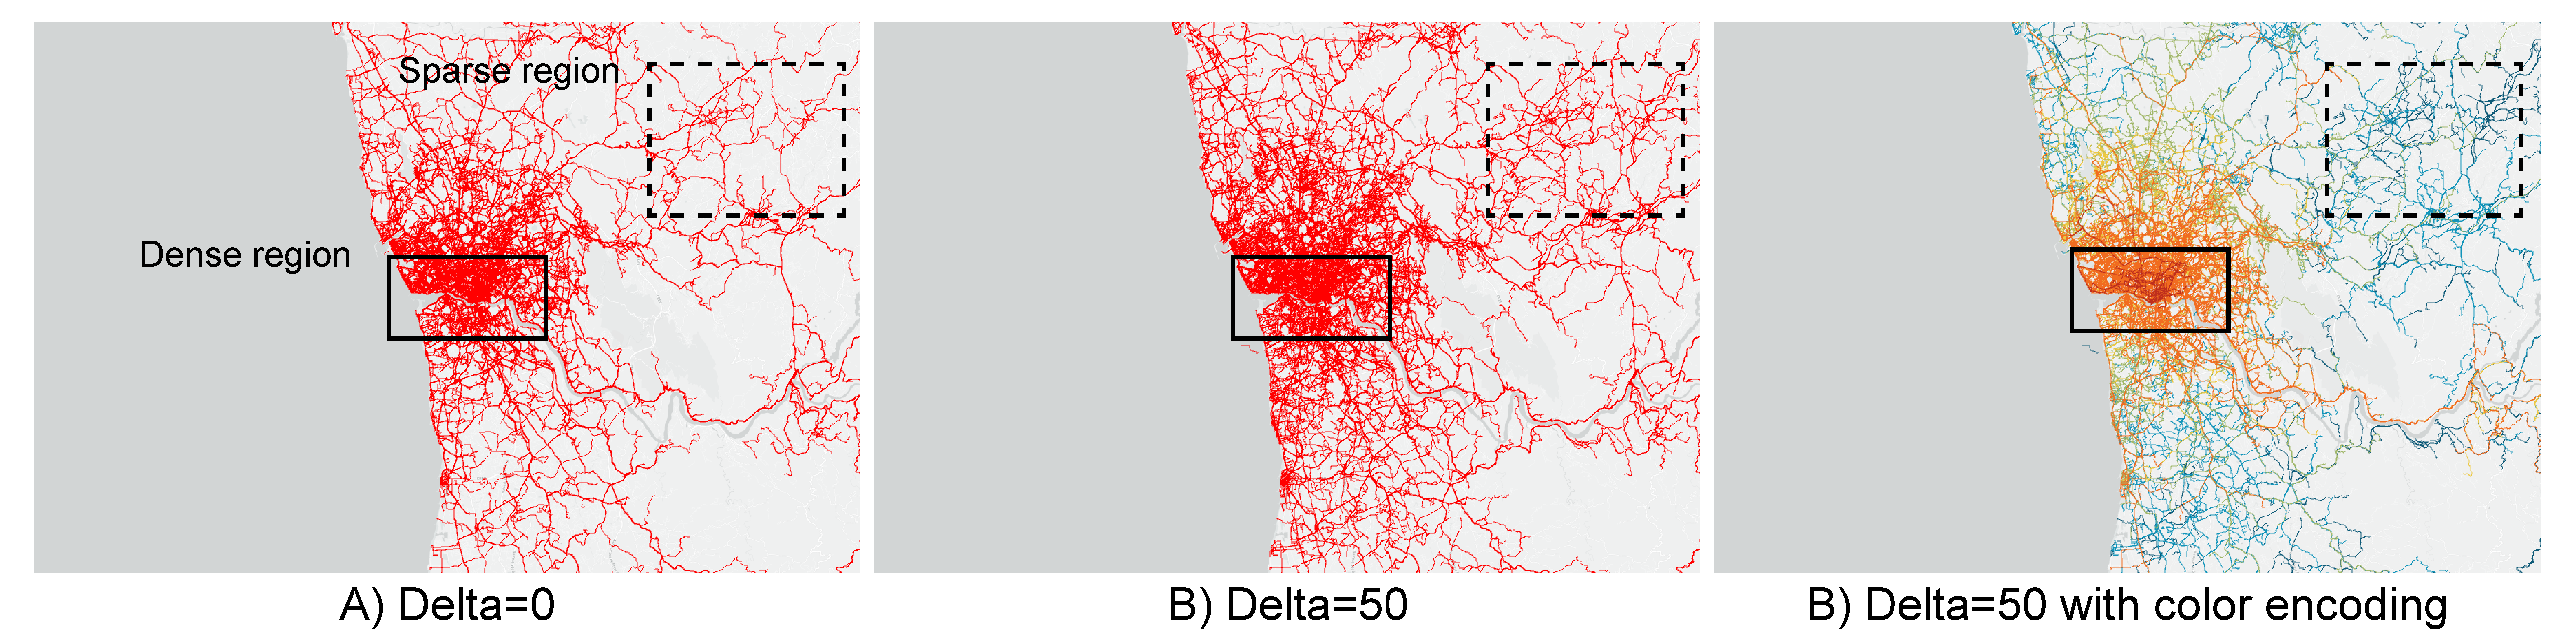
\includegraphics[width=0.95\textwidth]{pictures/problemsolveing/delta_motivation.pdf}
	\caption{Detail-aware visual quality guaranteed trajectory sampling, A: $\vats{}$, B: advanced $\vats$ ($\avats$), C: $\avats$ and popularity encoded by color.}
	\label{fig:delta}
\end{figure*}


\begin{figure}
 \centering
 \small
 \begin{tabular}{cc}
   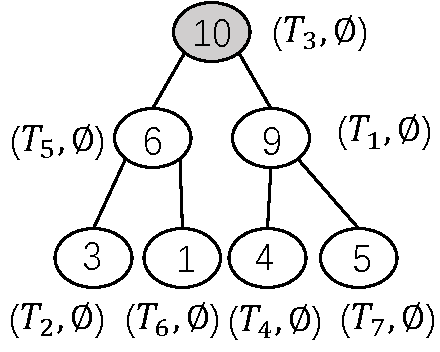
\includegraphics[width=0.46\columnwidth]{1st}
   &
   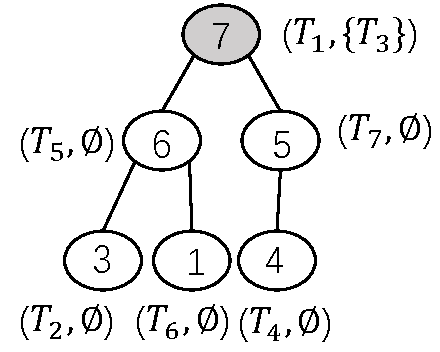
\includegraphics[width=0.46\columnwidth]{2nd}
   \\
   (a) 1st iteration
   &
   (b) 2nd iteration
 \end{tabular}
 \caption{Lazy updating manner illustration}
 \label{fig:heap}
\end{figure}



In summary, in the lazy updating manner, the number of uncovered pixels in each trajectory will only be computed with the latest result set $\oR$ when it is necessary,
e.g., only $\D_1$ will be updated at the 2nd iteration in Figure~\ref{fig:heap}.
It reduces many unnecessary computations through the lazy updating manner, e.g., all white nodes did not update at the 2nd iteration in the above example.
We analyze the time complexity of Algorithm~\ref{alg:greedy} with lazy updating manner in Theorem~\ref{lem:lazy}.

\begin{lemma}[Optimized Time Complexity]~\label{lem:lazy}
Given trajectory dataset $\D$ and an integer $k$, the time complexity of Algorithm~\ref{alg:greedy} with lazy updating manner is $O(|\D| + k \cdot m \cdot t \log |\D|)$, where $t$ is the maximum number of updating among all $k$ iterations and $t \ll |\D|$.
\end{lemma}

\begin{proof}
It first takes $O(|\D|)$ time to construct the max-heap.
Then, it incurs $O( m \cdot t \log |\D|)$ cost to select the trajectory with maximum uncovered pixels at each iteration ($k$ iterations in total).
Hence, the overall cost is $O(|\D| + k \cdot m \cdot t \log |\D|)$.
\end{proof}

\Bo{To exemplify, Algorithm~\ref{alg:greedy} costs 2.3 hours to return the results on Lisbon taxi trajectory dataset.
However it only takes 3.2 seconds with lazy updating manner.}

%\subsection{One-to-many strategy}~\label{sec:one_to_many}
%Since we detect the covered pixels in the highest level, two trajectories may be very close to each other but share very few pixels, which will lead to more information loss in the low zoom view as figure~\ref{fig:one_to_many}.
%We next elaborate a ``one-to-many'' strategy to further optimize the visual quality of our proposed technique.
%Recalling we use the highest zoom level to define the pixel size in the canvas.
%Thus, our visual quality guaranteed sampling algorithm is zoom-level oblivious, e.g., it guarantees the visual quality of result set $\oR$ at every zoom level.
%However, users always do not use/need the highest zoom level in visualization applications.
%For example, Google map shows city and streets at zoom level 1 and 15, respectively~\footnote{\url{https://developers.google.com/maps/documentation/}}.
%Motivated by the above observation, we devise ``one-to-many'' strategy by introducing a visual tolerance parameter $\delta$ to optimize the visual quality for users.
%Specifically, suppose the pixel with location $(x,y)$ in canvas is covered by result set $\oR$,
%the ``one-to-many'' strategy will ignore all the pixels around $(x,y)$ within $\delta$ offset distance, i.e., all pixels from $(x-\delta, y-\delta)$ to $(x+\delta, y+\delta)$ will be skipped.
%We will demonstrate the effectiveness of the visual tolerance $\delta$ in experimental evaluations.
%
%%https://developers.google.com/maps/documentation/maps-static/dev-guide#Zoomlevels
%\begin{figure}[t]
%	\centering
%	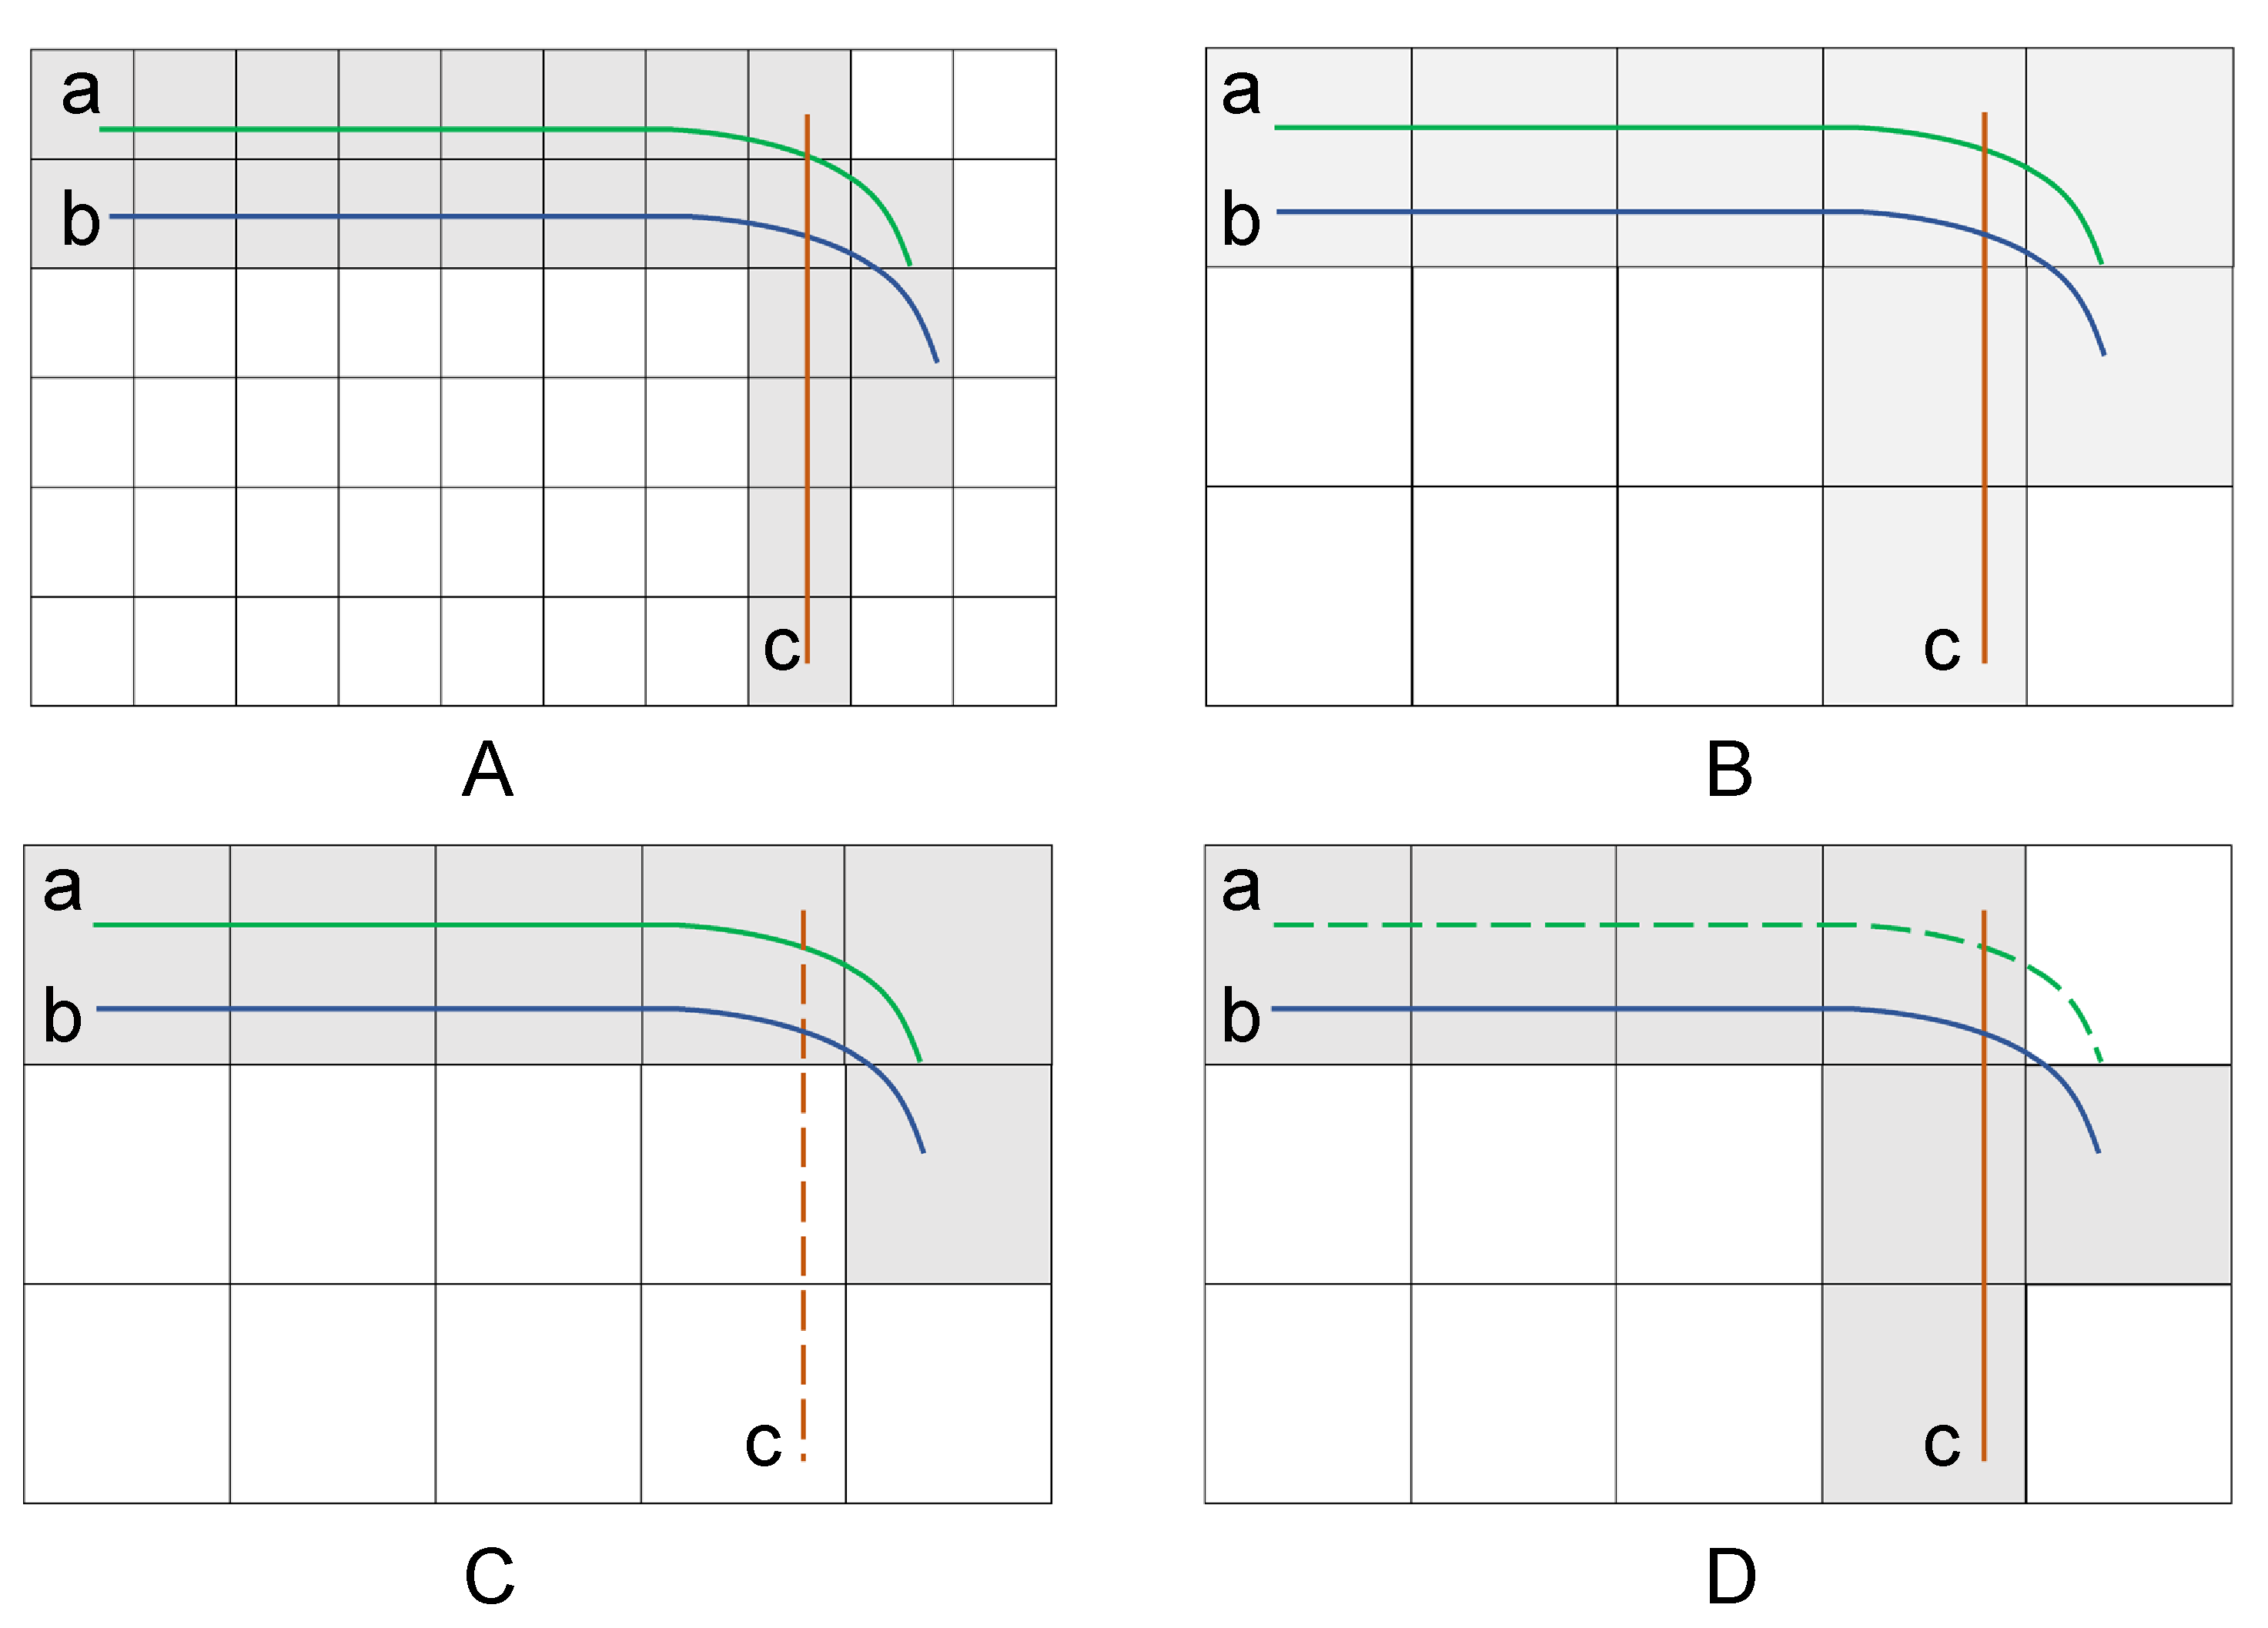
\includegraphics[width=0.4\textwidth]{pictures/problemsolveing/one_to_many.pdf}
%	\vspace{-5mm}
%	\caption{Resolution inconsistency}
%	\vspace{-5mm}
%	\label{fig:one_to_many}
%\end{figure}


% several notes for Bo, we should confirm them before submission:
% (1) rendering time,
% (2) gleaning insight from overview figures, i.e., low zoom level
% (3) delivers significantly richer information
% (4) arbitrary zooming resolutions





\section{Advance Approach: $\avats$}


Even though our proposed visual quality guaranteed sampling $\vats$ produces good quality visualization result for large trajectory dataset when comparing with random sampling method.
In this section, we devise an advanced $\vats$ (i.e., $\avats$) to further enhance the visual quality of $\vats$ by exploiting
(i) the inherent characteristic in the large trajectory dataset, and (ii) the interpretation ability of human beings.

We then elaborate (i) and (ii) by the examples in Figure~\ref{fig:delta}.
Considering Lisbon trajectory dataset, Figure~\ref{fig:delta}(a) shows its visualization result of $\vats$ with sampling ratio $1\%$.
The distribution of real-world trajectory dataset is non-uniform inherently.
For example, the dense region (Lisbon downtown) has much more trajectories than the sparse region in Figure~\ref{fig:delta}(a).
Obviously, it is much easier for us to distinguish the difference between sparse regions rather than dense regions in Figure~\ref{fig:delta}(a) and (b).
The major reason is that end users will treat the two dense regions in Figure~\ref{fig:delta}(a) and (b) as identical
since the interpretation ability of human beings is limited at such level of details.
However, the visual difference between the two sparse regions in Figure~\ref{fig:delta}(a) and (b) at that level of details is in the range of ours interpretation ability.

Hence, the returning result of visual quality guaranteed sampling method $\vats$ could be further improved by delivering richer information at sparse regions, 
i.e., enhancing the visual details in the region where is in the range of end user's interpretation ability.
We devise an advance approach $\avats$ by incorporating a parameter $\delta$ during trajectory selection process in $\vats$ to achieve the above objective.
In particular, we employ the parameter $\delta$ to model the end user's interpretation ability at the most high level of details.
Surprisingly, our advance approach $\avats$ not only provides better visualization result when compare with $\vats$ with the same sampling rate
(e.g., Figure~\ref{fig:delta}(a) and (b) are the returning result of $\vats$ and $\avats$ respectively
but also reveals the trajectory popularities by encoding it with colors (e.g., Figure~\ref{fig:delta}(a) is the visual result of $\avats$ with color encoded popularity).







%(1) Richer Information Delivering: details aware; so Arbitrary zooming resolutions
%(2) Popularity Embedding: visual clutter








